% !TeX TXS-program:compile = txs:///lualatex

\documentclass[a4paper,11pt]{article}
\usepackage[revgoku]{cp-base}
\graphicspath{{./graphics/}}
%variables.
\donnees[classe={1\up{ère} 2M2},matiere={[SPÉ.MATHS]},mois={Jeudi 2 Décembre},annee=2021,typedoc=TEST~,numdoc=3,duree={20 minutes}]
%formatage
\author{Pierquet}
\title{\nomfichier}
\hypersetup{pdfauthor={Pierquet},pdftitle={\nomfichier},allbordercolors=white,pdfstartview=FitH}
%divers
\lhead{\entete{Durée : \duree}}
\chead{\entete{\lycee}}
\rhead{\entete{\classe{} - \mois{} \annee}}
\lfoot{\pied{\matiere}}
\cfoot{\logolycee{}}
%\rfoot{\pied{\numeropagetot}}
\fancypagestyle{sujetA}{\fancyhead[R]{\entete{\classe{}A - \mois{} \annee}}}
\fancypagestyle{sujetB}{\fancyhead[R]{\entete{\classe{}B - \mois{} \annee}}}

\begin{document}

\pagestyle{fancy}

\part{TEST03 - Second degré, signes}

\setcounter{numexos}{0}

\medskip

\nomprenomtcbox

\medskip

\exonum{}

\medskip

Déterminer le signe des expressions suivantes :
%
\begin{enumerate}
	\item $-2x^2+6x+8$ :
	
	\medskip
	
	\begin{tikzpicture}
		\tkzTabInit[espcl=6]{$x$/0.8,expr/1.6}{$-\infty$,$+\infty$}
	\end{tikzpicture}~~~~
	\papierseyes*{10}{3}
	\item $3x^2-12x+12$ :
	
	\medskip
	
	\begin{tikzpicture}
		\tkzTabInit[espcl=6]{$x$/0.8,expr/1.6}{$-\infty$,$+\infty$}
	\end{tikzpicture}~~~~
	\papierseyes*{10}{3}
	\item $(2x-6)(x^2+x+1)$ :
	
	\medskip
	
	\begin{tikzpicture}
		\tkzTabInit[espcl=6]{$x$/0.8,$ $/0.8,$ $/0.8,expr/1.6}{$-\infty$,$+\infty$}
	\end{tikzpicture}~~~~
	\papierseyes*{10}{5}
\end{enumerate}

\smallskip

\exonum{}

\medskip

Résoudre l'inéquation $\dfrac{x^2-5x+6}{-x-4} \pg 0$.
%
\papierseyes{22}{4}

\end{document}